\documentclass{beamer}
\usetheme{Marburg}
\title{The Code That Never Ran: Modeling Attacks on Speculative Evaluation}
\author{Craig Disselkoen \and Radha Jagadeesan \and Alan Jeffrey \and James Riely}

\definecolor{bottle}{rgb}{0,0.45,0.35}
\setbeamercolor{sidebar}{bg=bottle}
\setbeamercolor{frametitle}{fg=bottle}
\setbeamercolor{section in toc}{fg=bottle!50!black}
\setbeamercolor{author in sidebar}{fg=bottle!50!white}
\setbeamercolor{itemize item}{fg=bottle}
\setbeamertemplate{sidebar canvas right}[vertical shading][top=black,bottom=bottle]

\usepackage{../doc/macros}

\begin{document}

\begin{frame}[plain]
  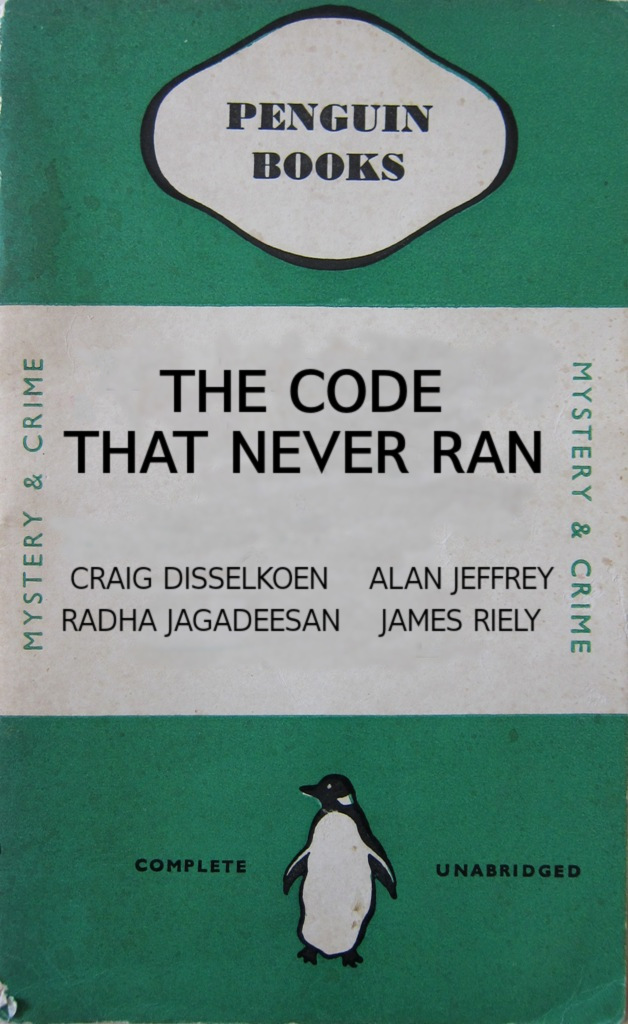
\includegraphics[height=.9\textheight]{green-penguin.jpg}
  \begin{minipage}[b][.9\textheight]{.66\textwidth}\raggedleft
    A classic locked-room mystery.\\
    Eve was in the false branch of a conditional the whole time,\\
    \emph{how could she do it}?

    \vss

    \tiny
    
\includegraphics[height=1.5ex]{cc-by-88x31.png}~Creative Commons Attribution-ShareAlike 4.0

    Mozilla Research \textbar~DePaul University \textbar~U.~California San Diego
  \end{minipage}
\end{frame}

\section{Introduction}
\begin{frame}{Overview}
  \begin{quotation}
  \tableofcontents
  \end{quotation}
\end{frame}

\begin{frame}[fragile]
  \frametitle{Why? Spectre!}

  {\fboxrule=1ex\fboxsep=0pt\fbox{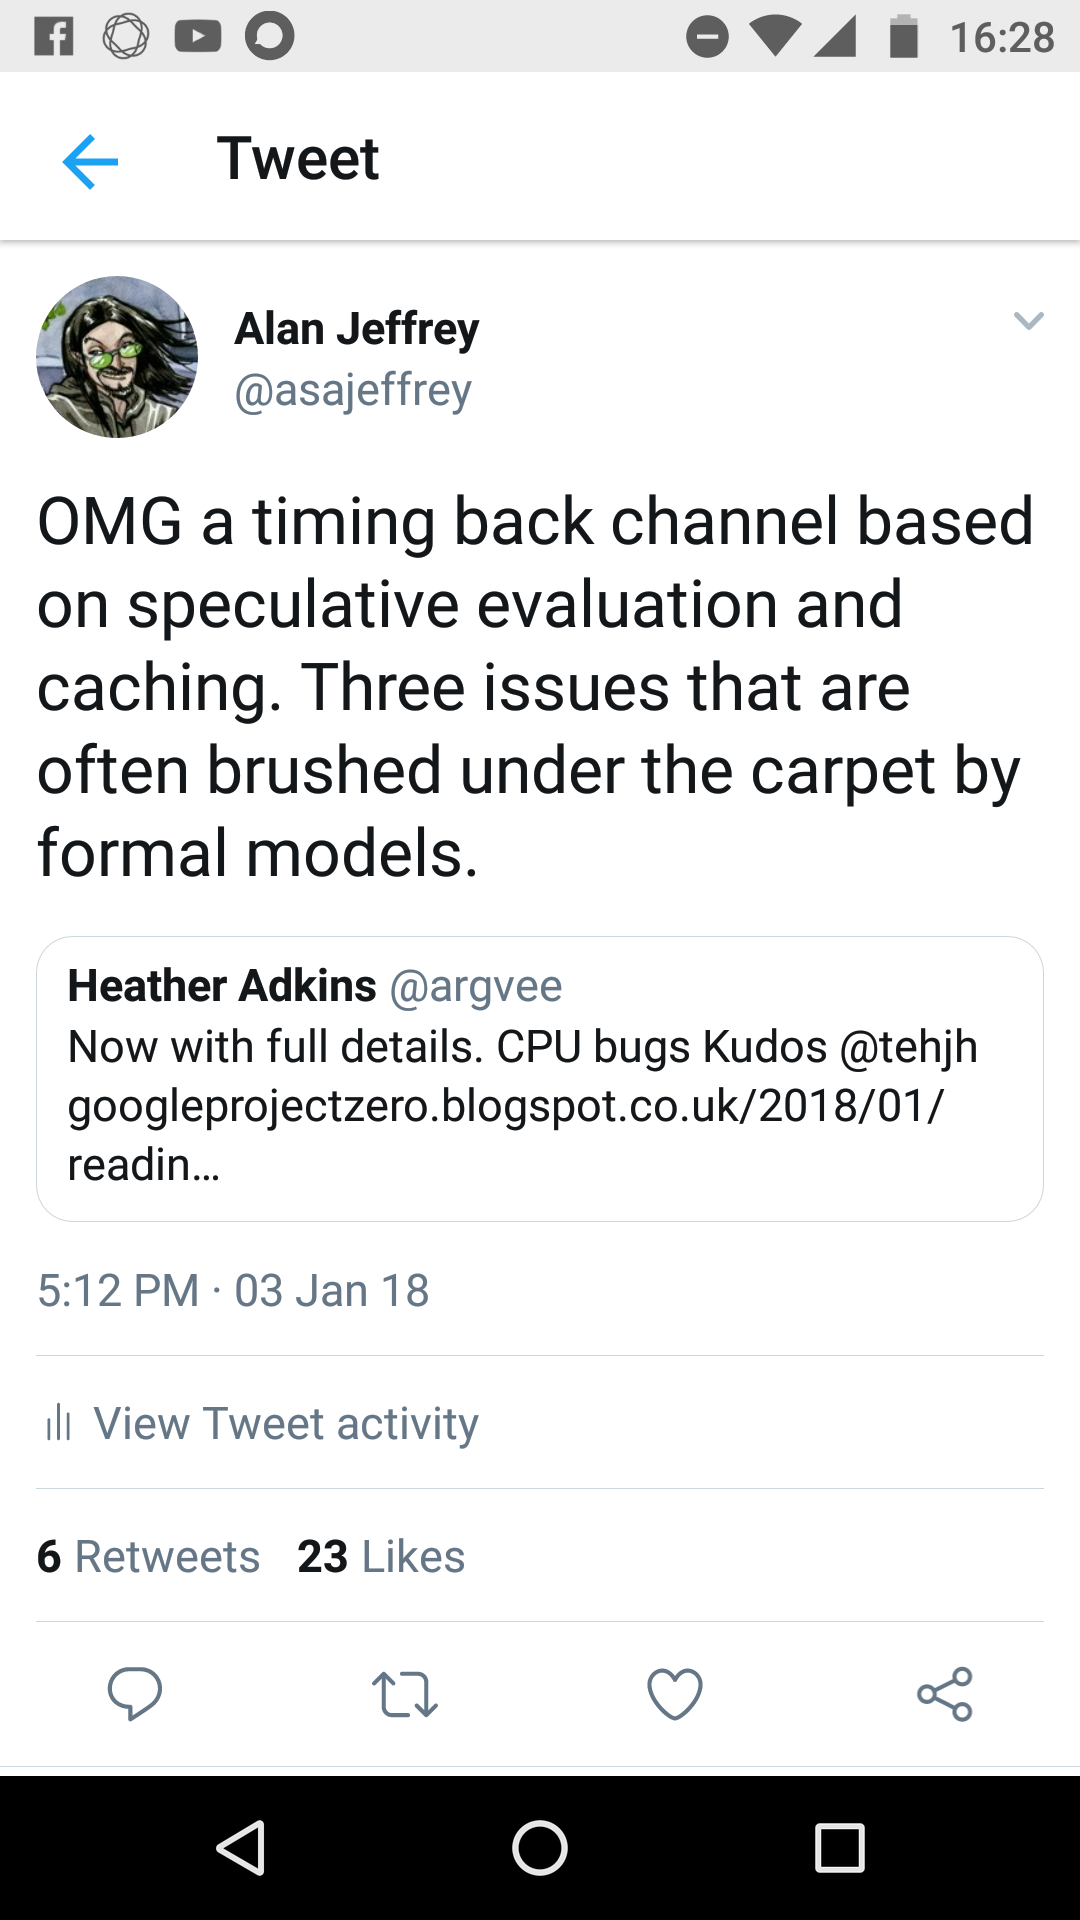
\includegraphics[height=.8\textheight]{omg-tweet.png}}}\quad\pause
  \begin{minipage}[b]{.45\textwidth}\raggedright
    Attacks bypass dynamic security checks:

\begin{verbatim}
if (canReadSecret) {
  doStuffWith(SECRET);
}
\end{verbatim}

    Information flow from \verb|SECRET|
    even though \verb|canReadSecret| is false.
    \bigskip

    Most formal models ignore code in branches
    that aren't taken.

    \bigskip
  \end{minipage}
\end{frame}

\begin{frame}
  \frametitle{Models that include speculation?}

  There are some models that include speculation\\
  \emph{relaxed memory models}:

  \begin{itemize}\footnotesize
  \item \emph{The Java Memory Model}\\
    Manson, Pugh and Adve, 2005.
  \item \emph{Generative Operational Semantics for Relaxed Memory Models}\\
    Jagadeesan, Pitcher and Riely, 2010.
  \item \emph{A promising semantics for relaxed-memory concurrency}\\
    Kang, Hur, Lahav, Vafeiadis and Dreyer, 2017.
  \end{itemize}

  \pause
  \emph{Question}: is there a simple model similar to
  those of relaxed memory, that can model speculation?
\end{frame}

\begin{frame}
  \frametitle{Information flow attacks on speculation}
  Speculation happens in many places:
  \begin{itemize}\footnotesize
  \item \emph{Speculation in hardware} (branch prediction,\ldots) \\
    \onslide<2->{Attacked by Spectre (Kocher \emph{et al.}~2019).}
  \item \emph{Transactions} (transactional memory,\ldots)\\
    \onslide<2->{Attacked by Prime+Abort (Disselokoen \emph{et al.}~2017).}
  \item \emph{Relaxed memory} (compiler optimizations,\ldots)\\
    \onslide<2->{No known attacks.}
  \end{itemize}
  
  \pause
  \emph{Question}: are there information flow attacks against
  compiler optimizations?
\end{frame}

\begin{frame}
  \frametitle{Contributions}
  \begin{itemize}\footnotesize
  \item A simple compositional model.
  \item Examples.
  \item Attacks (including a new attack on relaxed memory).
  \item Experiments (testing practicality of new attacks).
  \end{itemize}
\end{frame}

\section{Model}
\begin{frame}
  \frametitle{Pomsets}
  C11-style models are based on \emph{events} \\
  with \emph{labels} (e.g.~$(\DR{x}{3})$ or~$(\DW{x}{3})$)\\
  and \emph{relations} (e.g.~happens-before or reads-from).

  \bigskip\pause
  Simplest such is \emph{partially ordered multisets} (Gisher, 1988).

  \bigskip
  Only one relation, a partial order modelling dependency\pause, e.g.

\[\only<3>{\begin{tikzpicture}[node distance=1em]
  \event{rx1}{\DR{\aLoc}{1}}{}
  \event{wy1}{\DW{\bLoc}{1}}{right=of rx1}
  \event{wz2}{\DW{\cLoc}{2}}{right=of wy1}
  \po[out=25,in=155]{rx1}{wz2}
\end{tikzpicture}}
\only<4>{\begin{tikzpicture}[node distance=1em]
  \event{rx1}{\DR{\aLoc}{1}}{}
  \event{wy1}{\DW{\bLoc}{1}}{right=of rx1}
  \nonevent{wy2}{\DW{\bLoc}{2}}{below=of wy1}
  \po{rx1}{wy1}
  \po{rx1}{wy2}
\end{tikzpicture}}
\]

  \only<3>{is an execution of $(\aReg\GETS\aLoc\SEMI \bLoc\GETS1\SEMI \cLoc\GETS\aReg+1)$.}

  \only<4>{is an execution of $(\IF(\aLoc)\THEN \bLoc\GETS1 \ELSE \bLoc\GETS2 \FI)$.}
\end{frame}

\begin{frame}
  \frametitle{Compositional pomset model}

  First off, straight-line code.

  \pause\bigskip
  \emph{New idea}: put preconditions on events\pause, e.g.

\[\begin{tikzpicture}[node distance=1em]
  \onslide<5->{\event{rx1}{\DR{\aLoc}{1}}{}}
  \onslide<4->{\event{wy1}{\DW{\bLoc}{1}}{right=of rx1}}
  \onslide<3->{\event{wz2}{\only<3-4>{r=1\mid}\only<5>{1=1\mid} \DW{\cLoc}{2}}{right=of wy1}}
  \onslide<5->{\po[out=25,in=155]{rx1}{wz2}}
\end{tikzpicture}\]

  is an execution of $(\onslide<5->{\aReg\GETS\aLoc\SEMI} \onslide<4->{\bLoc\GETS1\SEMI} \cLoc\GETS\aReg+1)$.

  \bigskip
  \only<4>{\emph{Note}: no dependency because $\aReg$ does not depend on $\bLoc\GETS1$.}

  \only<5>{\emph{Note}: dependency because $\aReg$ depends on $\aReg\GETS\aLoc$.}

  \only<5>{\emph{Also note}: performing a substitution $[1/\aReg]$.}

  \only<6>{\emph{Visualize}: elide tautologies}
\end{frame}

\begin{frame}
  \frametitle{Compositional pomset model}

  Next, conditionals.

  \pause\bigskip
  \emph{New idea}: an execution of $\IF M \THEN \aCmd \ELSE \bCmd \FI$\\
  comes from an execution of $\aCmd$ \emph{and} an execution of $\bCmd$\pause, e.g.

\[\begin{tikzpicture}[node distance=1em]
  \onslide<6->{\event{rx1}{\DR{\aLoc}{1}}{}}
  \onslide<3,5->{\event{wy1}{\only<3,5>{\aReg\neq0 \mid}\only<6>{1\neq0 \mid} \DW{\bLoc}{1}}{right=of rx1}}
  \onslide<4-6>{\event{wy2}{\only<4,5>{\aReg=0 \mid}\only<6->{1=0 \mid} \DW{\bLoc}{2}}{below=of wy1}}
  \onslide<7>{\nonevent{nwy2}{\DW{\bLoc}{2}}{below=of wy1}}
  \onslide<6->{\po{rx1}{wy1}}
  \onslide<6>{\po{rx1}{wy2}}
  \onslide<7>{\po{rx1}{nwy2}}
\end{tikzpicture}\]

  is an execution of \((
    \onslide<6->{\aReg\GETS\aLoc\SEMI}
    \onslide<5->{\IF(\aReg)\THEN}
    \onslide<3,5->{\bLoc\GETS1}
    \onslide<5->{\ELSE}
    \onslide<4->{\bLoc\GETS2}
    \onslide<5->{\FI}
  )\)
  \only<3>{when $\aReg\neq0$}
  \only<4>{when $\aReg=0$}

  \bigskip
  \only<7>{\emph{Visualize}: elide tautologies and cross out unsatisfiables}

\end{frame}


\begin{frame}
  \frametitle{Compositional pomset model}

  But\dots\pause
  any execution of $\aCmd$ should be\\
  an execution of $\IF M \THEN \aCmd \ELSE \aCmd \FI$\pause, e.g.

\[\begin{tikzpicture}[node distance=1em]
  \event{rx1}{\DR{\aLoc}{1}}{}
  \event{wy1}{\DW{\bLoc}{1}}{right=of rx1}
  \nonevent{nwy1}{\DW{\bLoc}{1}}{below=of wy1}
  \po{rx1}{wy1}
  \po{rx1}{nwy1}
\end{tikzpicture}\]
  is an execution of $(\IF \aLoc\THEN \bLoc\GETS1 \ELSE \bLoc\GETS1 \FI)$\pause,
  but so is
\[\begin{tikzpicture}[node distance=1em]
  \event{rx1}{\DR{\aLoc}{1}}{}
  \event{wy1}{\DW{\bLoc}{1}}{right=of rx1}
\end{tikzpicture}\]

  \pause
  \emph{New idea}: events from different branches can merge.

\end{frame}

\begin{frame}
  \frametitle{Compositional pomset model}

  Lastly, concurrency.

  \bigskip\pause
  \emph{Old idea}: match reads with matching
  writes (\`a la C11)\pause, e.g.

\[\begin{tikzpicture}[node distance=1em]
  \event{ry1}{\DR{y}{1}}{}
  \event{wx1}{\DW{x}{1}}{below=of ry1}
  \event{rx1}{\DR{x}{1}}{right=2.5em of ry1}
  \event{wy1}{\DW{y}{1}}{below=of rx1}
  \po{ry1}{wx1}
  \rf{wx1}{rx1}
  \rf{wy1}{ry1}
\end{tikzpicture}\]

  is an execution of
\((
  x\GETS y \PAR r\GETS x\SEMI y \GETS 1
)\).

\end{frame}

\begin{frame}
  \frametitle{Compositional pomset model}

  Glossed over some details:
  \begin{itemize}\footnotesize
  \item 3-valued pomsets for negative constraints $d \ltN e$,
  \item sanity conditions on reads-from,
  \item precise rules for dependency,
  \item variable declaration,
  \item $\cdots$
  \end{itemize}
  All in the paper!
  
\end{frame}

\section{Examples}
\begin{frame}
  \frametitle{Examples go here}
\end{frame}

\section{Attacks}
\begin{frame}
  \frametitle{Information flow attacks go here}
\end{frame}

\section{Experiments}
\begin{frame}
  \frametitle{Implementing the new attacks}
\end{frame}

\section{Conclusions}
\begin{frame}
  \frametitle{Outro goes here}
\end{frame}

\end{document}
